%\renewcommand{\thechapter}{3}
\chapter{Gandalf}
\label{chap:gandalf}

\section{Introduction}
    We have developed a new code called \Gand\ \footnote{The code solves for
    \textit{$g$-and-Alf}v\'{e}n waves, hence the name.} to solve the KRMHD
    \eqsand{intro:krmhd:els}{intro:krmhd:gpm}. \Gand\,
    is written in CUDA, a GPU computing platform and programming model invented by NVIDIA,
    and is an efficient numerical tool to study the long-wavelength asymptotic behavior
    of anisotropic magnetized plasmas.

\section{Equations}
    
     Instead of directly solving \eqref{intro:krmhd:gpm}, we first expand $g$ in
     \eqref{intro:krmhd:gpm} (superscripts will be suppressed whenever no confusion would
     result) in terms of its Hermite moments. Evolving
    the moments of $g$ instead of using a grid in velocity space makes the numerical
    scheme spectrally accurate in the $\vpar$ coordinate. 
    Expanding \eqref{intro:krmhd:gpm} in terms of Hermite polynomials also provides an
	elegant analytical framework to study phase mixing (see
	\chapref{chap:phmixlin} for details).
    The Hermite moments are defined as follows:
    \beq
    g(\vpar) = \sum_{m=0}^\infty \frac{H_m (\vpar/\vth) F_0 }{\sqrt{2^m m!}} g_m, \quad
    g_m = \int \rmd \vpar\, \frac{H_m(\vpar/\vth)}{\sqrt{2^m m!}}\, g(\vpar), 
    \eeq
    where $H_m$ is the Hermite polynomial of order $m$. \Eqref{intro:krmhd:gpm} then becomes a
    fluid-like hierarchy of equations:
    \begin{align}
        \label{gandalf:eq:g0}
        &\od{g_0}{t} + \vth \nabla_\parallel\frac{g_1}{\sqrt{2}}  = 0, \\
        \label{gandalf:eq:g1}
        &\od{g_1}{t} + \vth \nabla_\parallel\lt(g_2 + \frac{\lt(1-1/\Lambda\rt)}{\sqrt{2}}\,g_0\rt)
        = 0,\\
        &\od{g_m}{t} + \vth \nabla_\parallel\lt(\sqrt{\frac{m+1}{2}}\,g_{m+1} +
        \sqrt{\frac{m}{2}}\,g_{m-1}\rt) \nonumber \\
        &= C[g_m],  \quad m\ge2.
        \label{gandalf:eq:gmeq}
    \end{align}
    The first term on the right hand side of \eqref{intro:krmhd:gpm}, being proportional to 
    $H_1$, only appears in \eqref{gandalf:eq:g1}. The parallel
    streaming term couples each Hermite moment to the previous and the next moment\footnote{This is a result of the Hermite recurrence relation: $H_{m+1}(v) = 2 v
	H_m(v)- 2 m H_{m-1}(v)$.}. Dynamical coupling of different Hermite moments
    is the mathematical manifestation of linear phase mixing in Hermite space. 

    The right hand side of \eqref{gandalf:eq:gmeq} has a collision operator $C[g_m]$ that
    has been added to the kinetic \eqref{intro:krmhd:gpm}. Collisions are included in order to regularize the system at small velocity space scales. More
    importantly, they are also physically required to generate entropy and heat the 
    plasma---an exactly collisionless limit is unphysical.
    We choose a convenient collision operator, the Lenard--Bernstein 
    collision operator \cite{lenard58}, which in Hermite space looks like:
    \beq
        C[g_m] = - \nu m g_m,
    \eeq
    where $\nu$ is the collision frequency. The collision operator acts only on
    the second and higher Hermite moments, and hence, conserves particle number and
    momentum. This particular collision operator is also manifestly most effective for the highest
    moments retained, since $C[g_m] \propto m$.
    
    \Eqref{intro:krmhd:els} and
    \eqsdash{gandalf:eq:g0}{gandalf:eq:gmeq} are the equations that are
    implemented in \Gand.
    
\section{Normalization}

    We normalize the perpendicular spatial co-ordinates $x, y$ and the parallel spatial
    co-ordinate $z$, to independent arbitrary length scales $\rho$ and $L$, respectively
    (with the assumption $L \gg \rho$). By normalizing parallel and perpendicular
    co-ordinates independently, we can simulate highly anisotropic fluctuations with
    a numerical box that is roughly a cube. In addition, since the ratio $L/\rho$ is
    arbitrary, a single run simulates a whole range of problems with varying degrees of
    anisotropy.  
     Time is normalized to $L/v_A$. 
    The Elsasser fields $\xi^\pm$ are normalized to $\rho v_A$ (gradients of the Elsasser
    fields have units of velocity---see \eqref{intro:eq:PhiPsi}).  The Hermite moments $g_m$ of
	the perturbed
    distribution function $g$ are in arbitrary units. The Elsasser fields $\xi^\pm$, and
	the distribution function moments $g_m$
    are scaled up by a factor of $L/\rho$ so that all normalized terms have unity order of
    magnitude.
    
The normalized equations can then be written as, 
\begin{align}
    \pd{\nabla_\perp^2 \xi^\pm}{t} \mp \pd{\nabla_\perp^2 \xi^\pm}{z} & = - \frac{1}{2} \left[
    \{\xi^+, \nabla_\perp^2 \xi^- \} + \{\xi^-, \nabla_\perp^2 \xi^+ \} \mp \nabla_\perp^2
    \{\xi^+, \xi^-
    \} \right], \label{gandalf:eq:rmhd:norm}
\end{align}
\begin{align}
    \label{gandalf:eq:g0:norm}
    &\od{g_0}{t} + \sqrt{\beta_i} \nabla_\parallel\frac{g_1}{\sqrt{2}}  = 0,\\
    \label{gandalf:eq:g1:norm}
    &\od{g_1}{t} + \sqrt{\beta_i} \nabla_\parallel\lt(g_2 + \frac{1-1/\Lambda}{\sqrt{2}}\,g_0\rt)
    = 0,\\
    &\od{g_m}{t} + \sqrt{\beta_i} \nabla_\parallel\lt(\sqrt{\frac{m+1}{2}}\,g_{m+1} +
    \sqrt{\frac{m}{2}}\,g_{m-1}\rt) \nonumber \\
    &= -\nu m g_m,  \quad m\ge2,
    \label{gandalf:eq:gmeq:norm}
\end{align}
where
\beq
    \od{}{t} = \pd{}{t} + \lt\{\Phi,\ldots\rt\}, \quad \nabla_\parallel =
    \pd{}{z} + \lt\{\Psi,\ldots\rt\}, 
\eeq
\beq
    \Phi = \frac{\xi^+ + \xi^-}{2}, \quad \Psi = \frac{\xi^+-\xi^-}{2},
\eeq
and $\beta_i = 8\pi n_{0i} T_i/B_0^2$ is the ion plasma beta, $n_{0i}$ is the equilibrium ion density,
$T_i$ is the equilibrium ion temperature, and $B_0$ is the magnitude of the background
magnetic field.

\section{Algorithm}
    
    We solve \eqsdash{gandalf:eq:rmhd:norm}{gandalf:eq:gmeq:norm} using a pseudo-spectral scheme.
    The Elsasser fields $\xi^\pm$, and the Hermite moments $g_m$ are expressed in terms of
    Fourier modes. The nonlinear term is calculated in the real space by taking fast Fourier
    transforms using the CUDA FFT library. After transforming back
    to Fourier space, the nonlinear term is dealiased according to
    the Orszag $2/3^{\text{rd}}$ dealiasing rule \cite{orszag71}.
    The time
    integration for the linear term in \eqref{gandalf:eq:rmhd:norm} is done analytically using an
    integrating factor technique (discussed below); the nonlinear term is integrated using second-order
    Runge-Kutta scheme\footnote{This choice was made for ease of numerical implementation,
	and due to memory constraints on the GPU. 
    The unconditionally unstable nature of RK2
    is mollified by choosing a small time-step. The RK2 time-stepping scheme can be easily
	improved upon, which we hope to do in the near future.}.
    
    Consider the Fourier transform of \eqref{gandalf:eq:rmhd:norm},
    \beq
        \pd{\xi^\pm}{t} \mp i k_z \xi^\pm = \frac{1}{k_\perp^2} \lt[\text{NL}\rt],
    \eeq
    where $\lt[\text{NL}\rt]$ are all the nonlinear terms.
    The $k_x=0, k_y=0$ mode is
    decoupled from all the other Fourier modes, and is not included in our simulations. 
    Multiply throughout by
    $e^{-ik_z t}$,
    \beq
        \pd{\lt(\xi^\pm e^{\mp ik_z t}\rt)}{t} = e^{\mp i k_z t}\frac{1}{k_\perp^2}
        \lt[\text{NL}\rt]. \label{gandalf:eq:rmhd:int}
    \eeq
    \Eqsand{gandalf:eq:rmhd:int}{gandalf:eq:gmeq} are then discretized in time and solved as follows:
    \begin{enumerate}
        \item Take a half time-step:
            \beq
                \xi^{\pm, n+1/2} = e^{\pm i k_z \delta t/2} \xi^{\pm, n} 
                + e^{\pm i k_z \delta t/2}\frac{1}{k_\perp^2}\lt[\text{NL}\rt]^n,
            \eeq
            \beq
                g_0^{n+1/2} = g_0^n - \frac{\delta t}{2} 
                \lt[\lt\{\Phi^n, g_0^n\rt\} + 
                \frac{i k_z \sqrt{\beta_i}}{\sqrt{2}} g_1^n  
                + \sqrt{\beta_i}\lt\{\Psi^n, \frac{g_1^n}{\sqrt{2}}\rt\}\rt],
            \eeq
            \bea
                g_1^{n+1/2} = g_1^n - \frac{\delta t}{2} 
                \lt[\lt\{\Phi^n, g_1^n\rt\} + 
                i k_z \sqrt{\beta_i} \lt(g_2^n +
                \lt(1-1/\Lambda\rt)\frac{g_0^n}{\sqrt{2}}\rt)\rt. \nonumber \\
                \lt. + \sqrt{\beta_i}\lt\{\Psi^n, \lt(g_2^n +
                \lt(1-1/\Lambda\rt)\frac{g_0^n}{\sqrt{2}}\rt)\rt\}\rt],
            \eea
            \bea
                g_m^{n+1/2} = g_m^n - \frac{\delta t}{2} 
                \lt[\lt\{\Phi^n, g_m^n\rt\} + 
                i k_z \sqrt{\beta_i}\lt(\frac{\sqrt{m+1}}{2} g_{m+1}^n +
                \frac{\sqrt{m}}{2} g_{m-1}^n\rt) \rt. \nonumber \\
                \lt.
                + \sqrt{\beta_i}\lt\{\Psi^n, \lt(\frac{\sqrt{m+1}}{2} g_{m+1}^n +
                \frac{\sqrt{m}}{2} g_{m-1}^n\rt)\rt\}\rt],
            \eea
            where the superscript denotes the time index.
        \item Calculate nonlinear terms at the half time-step:
            \bea
                \lt[\text{NL}\rt]^{n+1/2} = - \frac{1}{2} 
                \lt[ \{\xi^{+,n+1/2}, \nabla_\perp^2 \xi^{-, n+1/2} \} + \{\xi^{-,n+1/2},
                \nabla_\perp^2 \xi^{+,n+1/2} \}  \rt. \nonumber \\
                \lt.  \mp \nabla_\perp^2 \{\xi^{+,n+1/2}, \xi^{-,n+1/2} \} \rt].
            \eea
        \item Take a full time-step using the nonlinear term calculated in the previous
        step:
            \beq
                \xi^{\pm, n+1} = e^{\pm i k_z \delta t} \xi^{\pm,n} + e^{\pm i k_z \delta
                t}\frac{1}{k_\perp^2} \lt[\text{NL}\rt]^{n+1/2}.
            \eeq
            \beq
                g_0^{n+1} = g_0^n - \delta t
                \lt[\lt\{\Phi^{n+1/2}, g_0^{n+1/2}\rt\} + 
                \frac{i k_z \sqrt{\beta_i}}{\sqrt{2}} g_1^{n +1/2}
                + \sqrt{\beta_i}\lt\{\Psi^{n+1/2}, \frac{g_1^{n+1/2}}{\sqrt{2}}\rt\}\rt],
            \eeq
            \bea
                g_1^{n+1} = g_1^n - \delta t 
                \lt[\lt\{\Phi^{n+1/2}, g_1^{n+1/2}\rt\} + 
                i k_z \sqrt{\beta_i} \lt(g_2^{n+1/2} +
                \lt(1-1/\Lambda\rt)\frac{g_0^{n+1/2}}{\sqrt{2}}\rt)\rt. \nonumber \\
                \lt. + \sqrt{\beta_i}\lt\{\Psi^{n+1/2}, \lt(g_2^{n+1/2} +
                \lt(1-1/\Lambda\rt)\frac{g_0^{n+1/2}}{\sqrt{2}}\rt)\rt\}\rt], \nonumber \\
            \eea
            \bea
                g_m^{n+1} = g_m^n - \frac{\delta t}{2} 
                \lt[\lt\{\Phi^{n+1/2}, g_m^{n+1/2}\rt\} + 
                i k_z \sqrt{\beta_i}\lt(\frac{\sqrt{m+1}}{2} g_{m+1}^{n+1/2} +
                \frac{\sqrt{m}}{2} g_{m-1}^n\rt) \rt. \nonumber \\
                \lt.
                + \sqrt{\beta_i}\lt\{\Psi^{n+1/2}, \lt(\frac{\sqrt{m+1}}{2}
                g_{m+1}^{n+1/2} +
                \frac{\sqrt{m}}{2} g_{m-1}^{n+1/2}\rt)\rt\}\rt]. \nonumber \\
            \eea
         \item Integrate the dissipative terms (collisions and diffusion) using the same
         integrating factor technique as above:
            \beq
                \xi^\pm \to \xi^\pm \exp\lt(- \eta k_\perp^2 \delta t\rt),
            \eeq
            \beq
                g_0 \to g_0 \exp\lt(-\eta k_\perp^2 \delta t \rt), \quad g_1 \to g_1
                \exp\lt(-\eta k_\perp^2 \delta t \rt),
            \eeq
            \beq
                g_m \to g_m \exp\lt(-\eta k_\perp^2 \delta t - \nu m \delta t \rt), \quad
                m\geq 2.
            \eeq
            
    \end{enumerate}
    Since each Hermite moment is coupled to the next one, a suitable closure is required
    for the last retained Hermite moment, $g_M$. Two simple closures have been
    implemented: $g_{M+1} = 0$ and $g_{M+1}=g_{M-1}$. When the collisions are set high
    enough so that there is negligible energy in the last Hermite moment, the results are
    independent of the particular choice of closure. Throughout this thesis, we use the
    $g_{M+1}=0$ closure, along with finite collisions.
    
    Due to the explicit nature of the numerical scheme, the time step is restricted by a
    Courant-Friedrichs-Lewy condition:
    \beq
        \delta t = \frac{C}{\sqrt{M}}\times\text{Min}\lt\{\frac{1}{k_{x,\text{max}} \text{Max}\lt\{\lt|k_y
        \xi^\pm\rt|\rt\}},
        \frac{1}{k_{y,\text{max}} \text{Max}\lt\{\lt|k_x \xi^\pm\rt|\rt\}}\rt\},
    \eeq
    where $C$ is a positive constant less than one, specified by the user.

\section{Additional features}
    %In this section, we list the additional features included in \Gand.

    \subsection{Forcing}
        
        A Gaussian white noise source has been implemented in order to study driven
        turbulence. The two Elsasser fields are driven
        using the same source---this ensures that only the velocity field
        $\mb{u}_\perp = \hat{\mb{z}}\times \nabla \Phi$ is forced, and there is no
        artifical large-scale reconnection. The slow modes are driven independently by
        forcing the zeroth and/or the first moment. 
        The slow modes can also be be driven by injecting energy into the field strength
        fluctuations---this physically corresponds to an external antenna that 
        drives a perpendicular current in the plasma. The slow modes are driven at
        specified wavenumbers $(k_x, k_y, k_z)$\footnote{Due to the Alfv\'{e}nic turbulence, the
        total magnetic field is not the same as the background magnetic field, $\mb{B} =
        B_0\hat{\mb{z}} + \delta \mb{B}_\perp$. As a result, the wavenumber $k_z$ is not
        necessarily same as the wavenumber along the total field $k_\parallel$. The
        implemented forcing routine does not check for what $\kpar$ values are being
        forced.}.






    \subsection{Hyper-dissipation}
    \label{gandalf:sec:hyper}
       
       Theories of turbulence generally give predictions for wavenumbers far from forcing
       and disipation scales, \ie, in the inertial range.
       The range of such wavenumbers may be estimated
       roughly as the ratio between the forcing and the dissipation scales, and hence is
       limited by resolution constraints. To maximize this range, we employ
       hyper-diffusion ($-\eta k_\perp^{2r}$) and hyper-collisions ($-\nu m^{2n}$) instead
       of regular diffusion ($-\eta k_\perp^2$) or collisions ($-\nu m$); 
       $r$ and $n$ are positive integers. Such hyper-dissipation operators restrict the
       dissipation range to a very narrow set of wavenumbers, and help the user simulate a
       large inertial range at a lower computational cost \cite{basdevant81,meneguzzi81,
       mcwilliams84,passot88jcp,borue95}. Typically, in this thesis, $r=4$ and $n=4$ were
       used. For the KRMHD simulations in \chapref{chap:slowmodes}, $r=8$ was used.
       
    \subsection{Diagnostics}
        
        \Gand\ writes out the following diagnostic data every few time-steps:
        \begin{itemize}
            \item For the Alfv\'{e}nic fluctuations, we calculate the kinetic~$\lt|k_\perp^2 \Phi^2\rt|$ and 
            magnetic~$\lt|k_\perp^2 \Psi^2 \rt|$ energy spectra as functions of $k_\perp$ and
            $\kpar$. For slow modes, the energy spectrum $\lt|g_m^2\rt|$ is a function of $k_\perp$, $\kpar$
            and $m$. 
            
            Energy at a particular perpendicular wavenumber $k_\perp = \sqrt{k_x^2 +
            k_y^2}$ is calculated by summing over shells. A mode at $k_x, k_y$
            contributes to the spectrum at $k_\perp$, if and only if, $k_\perp-0.5 \leq
            \sqrt{k_x^2 + k_y^2} < k_\perp+0.5$. The wavenumber $\kpar$, is the parallel
            wavenumber calculated along
            the local mean field. That is to say, $\kpar$ includes the perpendicular
            perturbation:
            \beq
                \hat{\mb{b}}\cdot\nabla = \pd{}{z} + \lt\{\Psi,\ldots\rt\},
                \label{gandalf:eq:parder}
            \eeq
            and is not same as $k_z$. The distinction between $k_z$ and $\kpar$ is
            important, because the two terms in
            \eqref{gandalf:eq:parder} appear at the same
            order in the gyrokinetic ordering. Since particles are not aware of the split
            between the background and fluctuating magnetic fields, and always experience
            the total magnetic field,
            $\kpar$ is the more physical choice for a parallel wavenumber.
            We calculate the $\kpar$ dependence of the spectra by following the exact
            field lines through our numerical box, and interpolating fluctuations along
            these field lines. This is done as follows:
            \begin{enumerate}
                \item Transform all the fluctuations from Fourier space to real space.

                \item Pick an initial position $x_0, y_0$ at one end of the box, say
                $z_0= - Lz/2$, where $L_z$ is the length of the box in the $z$ direction.

                \item Calculate the perturbations $\mb{u}_\perp =
                \hat{\mb{z}}\times\Phi$, $\mb{\delta B_\perp} =
                \hat{\mb{z}}\times\Psi$ and $g_m$  at $x~=~x_0, y~=~y_0, z~=~z_0$, using
                bilinear interpolation\footnote{This choice of interpolation scheme is
                sufficient for our purposes. A better scheme, like cubic splines could be
                easily implemented.}.

                \item Take a half step forward along the field line:
                    \beq
                        x_{1/2} = x_0 + \delta B_x\, \Delta z/2, \quad y_{1/2} = y_0 +
                        \delta B_y\, \Delta z/2, \quad z_{1/2} = z_0 + \Delta z/2,
                    \eeq
                    where $\Delta z = L_z/k_{z,max}$ is the spacing-in-$z$ between nearby grid
                    points in real space.

                \item Calculate the magnetic field perturbation $\mb{\delta B_\perp}$ at
                $x_{1/2}, y_{1/2}, z_{1/2}$ using bilinear interpolation.

                \item Take a full step forward along the field line using the value of the
                magnetic field at $x_{1/2}, y_{1/2}, z_{1/2}$:
                \beq
                        x_{1} = x_0 + \delta B_x\, \Delta z, \quad y_{1} = y_0 +
                        \delta B_y\, \Delta z, \quad z_{1} = z_0 + \Delta z.
                \eeq

                \item If $z_1 < L_z/2$, copy over the positions: $x_0 \gets x_1$, $y_0 \gets y_1$, $z_0
                \gets
                z_1$, and repeat from step 3.
                \item Once the fluctuations $\mb{u}_\perp$, $\delta \mb{B}_\perp$ and $g_m$ are
                known along the exact field lines, transform them back to Fourier space.
                The parallel wavenumber is this space is, in fact, $\kpar$.
                \item Calculate the spectra as functions of $k_\perp$ and $\kpar$ by
                summing over shells, as discussed above.
            \end{enumerate}

            A related, somewhat subtle issue is that of periodicity of the magnetic
            field lines. It is observed that the magnetic field lines that are initially
            periodic---say, for a driven simulation---naturally become aperiodic due to
            the turbulence. It can be shown that the $\kpar=0$ mode plays a crucial role
            in giving rise to this aperiodicity. However, we do not discuss this point
            further in this thesis.

            \item 
            The flux of energy $\Gmk$ from the $m^{\text{th}}$ to the $(m+1)^{\text{st}}$
            Hermite moment is calculated as
            \beq
                \Gmk = -\kpar\,\sqrt{2 (m+1)}\, \text{Im} \lt[g_{m+1} g_m^\star\rt].
            \eeq
            The derivation of this expression is discussed in detail in
            \secref{phmixlin:sec:flux}. 

            \item 
            For large values of $m$, a slow mode perturbation can be split into a phase mixing
            component that propagates from small to large $m$, and an phase unmixing
            component that propagates from large to small $m$ (see
            \secref{phmixlin:sec:cont}). In \Gand, we also calculate the spectra for these
            phase mixing and phase unmixing modes.
        \end{itemize}


\section{Code verification}
    
    %\subsection{Linear Landau damping of the ion acoustic wave}

    \subsection{Kinetic fluctuation-dissipation relations}

    In \chapref{chap:phmixlin}, we calculate the saturated amplitudes of a driven kinetic
    field that evolves according to the linearized Vlasov equation.
    The analytical predictions are compared with the numerical results obtained from
    \Gand\ in \figsand{phmixlin:fig:f}{phmixlin:fig:f1}. The comparison shows good agreement.

    \Figref{phmixlin:fig:Cpm} plots the phase mixing and phase unmixing spectra of the kinetic field versus $m$. The
    numerical spectra calculated using \Gand\ agree with the analytical
    prediction. The dotted lines in \figref{phmixlin:fig:Cpm} are not fits to the
    numerical spectra, but are the exact expressions from
    \eqsand{phmixlin:eq:Cuniv}{phmixlin:eq:Cminus}, \ie, the agreement between the
    numerics and the analytical predictions is not just for the scaling in $m$, but also
    for the overall level of the spectra.

    These comparisons provide a solid linear benchmark for \Gand.


    \subsection{Orszag-Tang test case}

    We present results from the well-known Orszag-Tang test case \cite{orszag79} for MHD
    simulations. The initial condition for this test is given by
    \beq
        \Phi = - 2\lt(\cos \lt(2\pi\frac{x}{L_x}\rt) +\cos\lt(2\pi\frac{y}{L_y}\rt)\rt),
    \eeq
    \beq
        \Psi = \lt(\cos\lt(4 \pi \frac{x}{L_x}\rt) + 2 \cos\lt(2 \pi
        \frac{y}{L_y}\rt)\rt).
    \eeq

    We evolved this initial condition for two Alfv\'{e}n times, using a $32^2\times 1$
    sized simulation domain. \Figref{gandalf:fig:OTenergy} plots the time evolution of kinetic and magnetic
    energies for the above initial condition, which is in qualitative agreement with the
    original results by Orszag and Tang. 

        \begin{figure}
            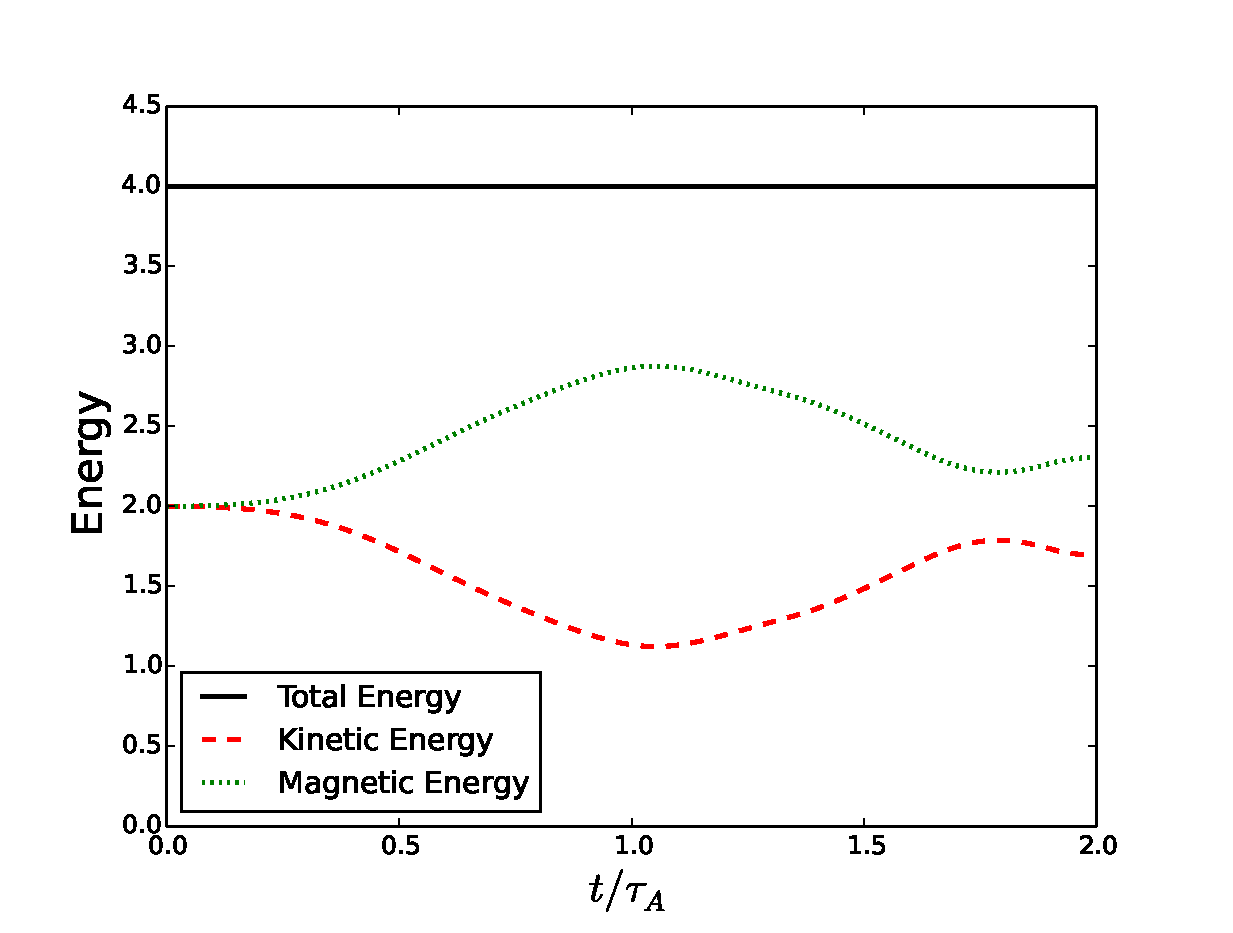
\includegraphics[width=14.8cm]{figs/gandalf/OT_energy.eps}
            \caption{Time evolution of kinetic and magnetic energies for the Orszag-Tang
            test case.}
            \label{gandalf:fig:OTenergy}
        \end{figure}

    \subsection{Turbulent spectra for Alfv\'{e}nic cascade}
    
    \begin{figure}
    \begin{center}
        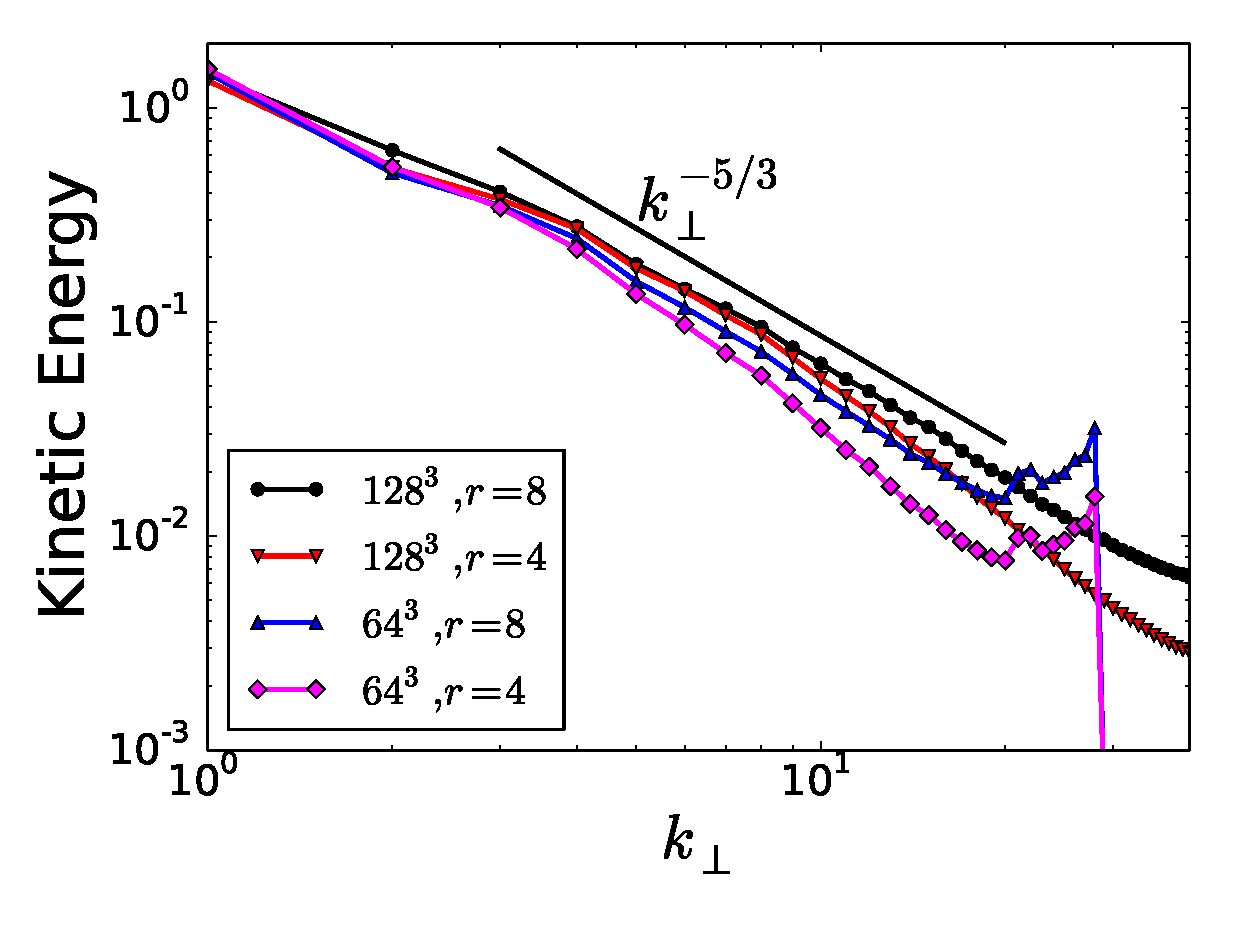
\includegraphics[width=7.4cm]{figs/gandalf/alfconv_KE.eps}
        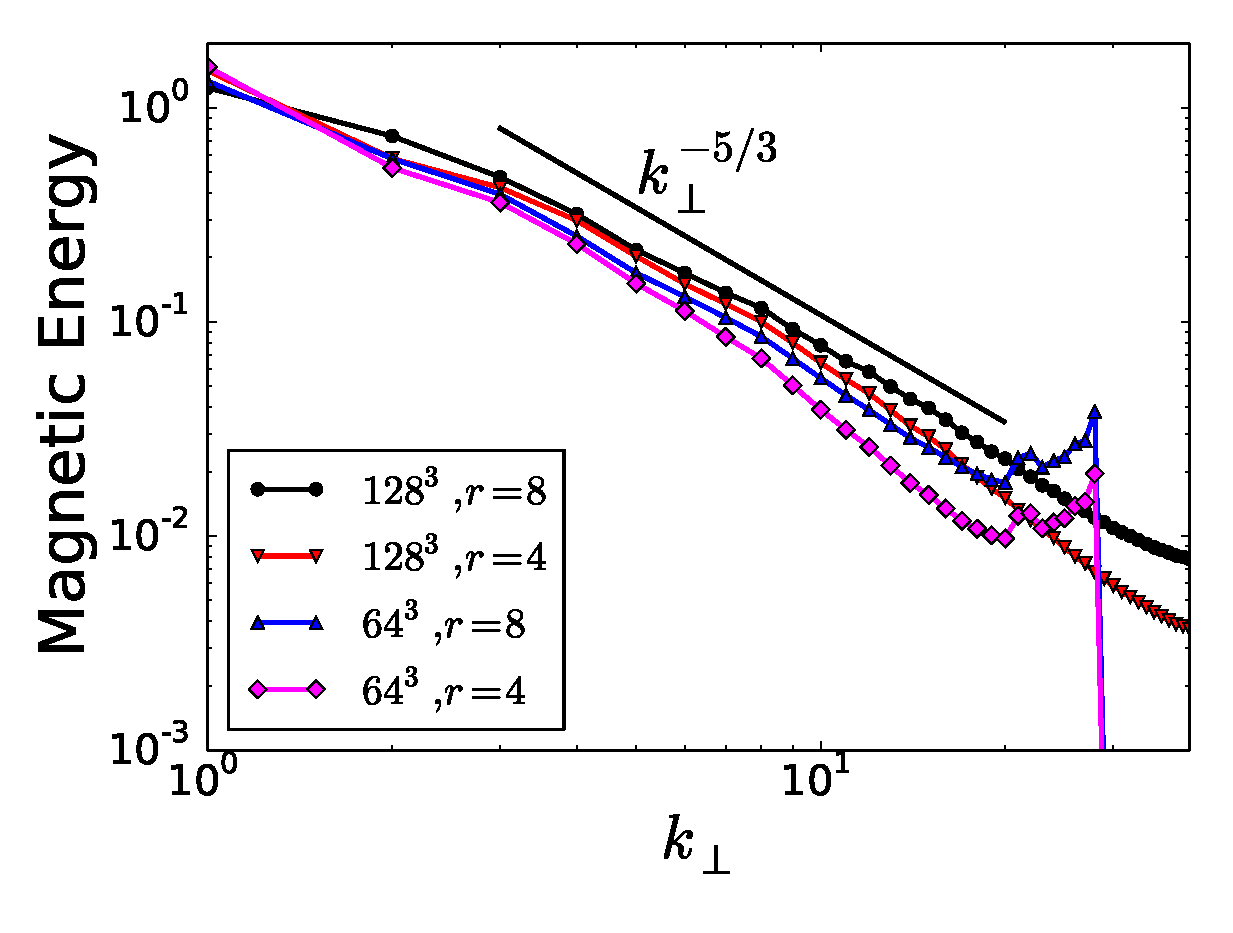
\includegraphics[width=7.4cm]{figs/gandalf/alfconv_ME.eps}
        \caption{The kinetic (left) and magnetic (right) energy spectra for Alfv\'{e}nic
        turbulent cascade. The four different lines correspond to four separate
        simulations---the first number is the resolution, and the second number is
        the exponent for the hyper-diffusion term (see \secref{gandalf:sec:hyper}). The
        spectra approach the critical-balance prediction of $k_\perp^{-5/3}$ for large
        resolution, and for large hyper-diffusion exponent.}
        \label{gandalf:fig:alfconv}
    \end{center}
    \end{figure}

    We simulated the reduced MHD equations for the simulation domains $64^3$, and $128^3$,
    with two different values for the hyper-diffusion exponent: $r=4$ and $r=8$. We ran
    these simulations till saturation, and then time-averaged the kinetic and magnetic
    energy spectra over two Alfv\'{e}n times. These time-averaged spectra are plotted in
    \figref{gandalf:fig:alfconv}---they are in agreement with the critical-balance prediction of
    $k_\perp^{-5/3}$.


